\documentclass{article}

% Document extensibility %
%
% Disables native paragraph indentation
\usepackage{parskip} 
%
% Provides further bullet options for lists
\usepackage{enumitem}

% Mathematical symbol and statement packages %
%
% Necessary
\usepackage{amsmath}
\usepackage{amssymb}
%
% Extensive fraction notation
\usepackage{xfrac}
%
% Generic mathematical commands
% Notable: \degree, \celcius
\usepackage{gensymb}
%
% Variable vector notation (arrow above variable)
\usepackage{esvect}
%
% Multiline boxed equations
\usepackage{empheq}
%
% SI Unit
\usepackage{siunitx}
\DeclareSIUnit{\north}{North}
\DeclareSIUnit{\south}{South}
\DeclareSIUnit{\west}{West}
\DeclareSIUnit{\east}{East}
\DeclareSIUnit{\of}{ of }
\DeclareSIUnit{\erg}{erg}
\usepackage{physunits}
%
% More intuitive arrays/matrices
\usepackage{array}
%
% Linear Equations
\usepackage{systeme}
%
% Boxes!
\usepackage{mdframed}
%
% Matrix Notation
\usepackage{bm}

% Graphic packages %
%
% Diagrams and illustrations
\usepackage{tikz}
\usetikzlibrary{positioning}
%
% Image insertion
\usepackage{graphicx}

% Document content %
%
% Change title of table of contents
% \renewcommand{\contentsname}{Title}

\title{Homework 8 - Momentum}
\author{Corey Mostero - 2566652}
\date{25 May 2023}

\begin{document}

% Command `\hr` to insert horizontal rules
\newcommand{\hr}{\par\noindent\rule{\textwidth}{0.4pt}}

% Command to box and center math equations
\newcommand{\bc}[1]{
	\begin{equation*}
		\begin{boxed}
			{#1}
		\end{boxed}
	\end{equation*}
}

% Command for single line equations with a condition
\newcommand{\cond}[2]{
	\ifmmode
		{#1} \quad {#2}
	\else
		$$ {#1} \quad {#2} $$
	\fi
}

% Matrix and Vector notation
\newcommand{\matr}[1]{
	\ifmmode \bm{#1}
	\else \textit{\textbf{#1}}
	\fi
}
\newcommand{\vect}[1]{
	\ifmmode \mathbf{#1}
	\else \textbf{#1}
	\fi
}

\maketitle
\newpage

\tableofcontents

\section{Book}

\subsection{8.16}

\begin{align*}
	m_{(a)stronaut} & = \SI{65.5}{\kilogram} \\
	m_{(t)ool} & = \SI{2.50}{\kilogram} \\
	v_{t_1} & = \SI{3.10}{\meter \per \second} \\
	v_{a_1} & = ?
\end{align*}
\begin{align*}
	P_0 & = P_1 \\
	m_av_{a_0} + m_tv_{t_0} & = m_av_{a_1} + m_tv_{t_1} \\
	0 + 0 & = m_av_{a_1} + m_tv_{t_1} \\
	v_{a_1} & = -\frac{m_tv_{t_1}}{m_a} \\
	v_{a_1} & = -\frac{(\SI{2.50}{\kilogram})(\SI{3.10}{\meter \per \second})}{\SI{65.5}{\kilogram}} \\
	v_{a_1} & = \SI{-0.118}{\meter \per \second}
\end{align*}
\begin{mdframed}
	The astronaut will move at a speed of \SI{0.118}{\meter \per \second} opposite of the tool's direction.
\end{mdframed}

\subsection{8.21}

\begin{align*}
	m_A & = \SI{0.245}{\kilogram} \\
	m_B & = \SI{0.360}{\kilogram} \\
	v_{B_0} & = 0 \\
	v_{A_1} & = \SI{-0.118}{\meter \per \second} \\
	v_{B_1} & = \SI{0.660}{\meter \per \second} \\
	v_{A_0} & = ?
\end{align*}
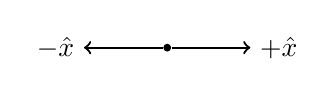
\begin{tikzpicture}
	\node [circle, fill, inner sep = 1pt] (origin) {};
	\node [left = of origin] (x0) {$ -\hat{x} $};
	\node [right = of origin] (x1) {$ +\hat{x} $};

	\foreach \node in {x0, x1}
		\draw[black, thick, ->] (origin) -- (\node);
\end{tikzpicture}
\begin{enumerate}[label = \textbf{(\alph*)}]
	\item What was the speed of puck $ A $ before the collision?
		\begin{align*}
			P_0 & = P_1 \\
			m_A v_{A_0} + m_B v_{B_0} & = m_A v_{A_1} + m_B v_{B_1} \\
			m_A v_{A_0} + 0 & = m_A v_{A_1} + m_B v_{B_1} \\
			v_{A_0} & = \frac{ m_A v_{A_1} + m_B v_{B_1} }{ m_A } \\
			v_{A_0} & = \frac{ (\SI{0.245}{\kilogram})(\SI{-0.118}{\meter \per \second}) + (\SI{0.360}{\kilogram})(\SI{0.660}{\meter \per \second}) }{ \SI{0.245}{\kilogram} } \\
			v_{A_0} & = \SI{0.852}{\meter \per \second}
		\end{align*}
		\bc{ v_{A_0} = \SI{0.852}{\meter \per \second} }
	\item Calculate the change in the total kinetic energy of the system that occurs during the collision.
		\begin{align*}
			\Delta PE & = E_{A_1} + E_{B_1} - E_{A_0} + E_{B_0} \\
			\Delta PE & = \frac{1}{2}m_Av_{A_1}^2 + \frac{1}{2}m_Bv_{B_1}^2 - \frac{1}{2}m_Av_{A_0}^2 + 0 \\
			\Delta PE & = \frac{1}{2}(\SI{0.245}{\kilogram})(\SI{-0.118}{\meter \per \second})^2 + \frac{1}{2}(\SI{0.360}{\kilogram})(\SI{0.660}{\meter \per \second})^2 \\
					  & - \frac{1}{2}(\SI{0.245}{\kilogram})(\SI{0.852}{\meter \per \second})^2 \\
			\Delta PE & = \SI{-0.00881}{\joule} = \SI{8.81e-3}{\joule}
		\end{align*}
		\bc{ \Delta PE = \SI{-0.00881}{\joule} = \SI{8.81e-3}{\joule} }
\end{enumerate}

\subsection{8.30}

\begin{align*}
	m_A = m_B & = ? \\
	v_{A_0} & = \SI{40.0}{\meter \per \second} \\
	\theta_A & = \SI{30.0}{\degree} \\
	v_{B_0} & = 0 \\
	\theta_B & = \SI{-45.0}{\degree} \\
	v_{A_1} & = ? \\
	v_{B_1} & = ?
\end{align*}
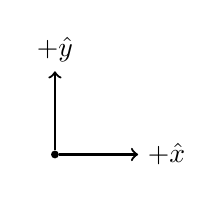
\begin{tikzpicture}
	\node [circle, fill, inner sep = 1pt] (origin) {};
	\node [above = of origin] (y) {$ +\hat{y} $};
	\node [right = of origin] (x) {$ +\hat{x} $};

	\foreach \node in {y, x}
		\draw[black, thick, ->] (origin) -- (\node);
\end{tikzpicture}
\begin{enumerate}[label = \textbf{(\alph*)}]
	\item Find the speed of each asteroid after the collision. \\
		Speed of asteroid in $ \hat{x} $ direction:
		\begin{align*}
			v_{A_0} & = \SI{40.0}{\meter \per \second}\cos(\SI{0}{\degree}) = \SI{40.0}{\meter \per \second} \\
			v_{B_0} & = 0 \\
			v_{A_1} & = v_{A_1}\cos(\SI{30.0}{\degree}) \\
			v_{B_1} & = v_{B_1}\cos(\SI{-45.0}{\degree})
		\end{align*}
		\begin{align*}
			P_{0_x} & = P_{1_x} \\
			m_Av_{A_0} + m_Bv_{B_0} & = m_Av_{A_1} + m_Bv_{B_1} \\
			v_{A_0} & = v_{A_1} + v_{B_1} \\
			\SI{40.0}{\meter \per \second} & = v_{A_1}\cos(\SI{30.0}{\degree}) + v_{B_1}\cos(\SI{-45.0}{\degree})
		\end{align*}
		Speed of asteroid in $ \hat{y} $ direction:
		\begin{align*}
			v_{A_0} & = \SI{40.0}{\meter \per \second}\cos(\SI{90}{\degree}) = 0 \\
			v_{B_0} & = 0 \\
			v_{A_1} & = v_{A_1}\sin(\SI{30.0}{\degree}) \\
			v_{B_1} & = v_{B_1}\sin(\SI{-45.0}{\degree})
		\end{align*}
		\begin{align*}
			P_{0_y} & = P_{1_y} \\
			m_Av_{A_0} + m_Bv_{B_0} & = m_Av_{A_1} + m_Bv_{B_1} \\
			0 & = v_{A_1} + v_{B_1} \\
			v_{A_1}\sin(\SI{30.0}{\degree}) + v_{B_1}\sin(\SI{-45.0}{\degree}) & = 0
		\end{align*}
		\begin{align*}
			\left[ \matr{A} | \vect{v} \right] & =
				\left[ \begin{array}{ c c | c }
					\cos(\SI{30.0}{\degree}) & \cos(\SI{-45.0}{\degree}) & \SI{40.0}{\meter \per \second} \\
					\sin(\SI{30.0}{\degree}) & \sin(\SI{-45.0}{\degree}) & 0
			\end{array} \right]
		\end{align*}
		\begin{align*}
			\matr{A}_2 & = \matr{A}_2 - \matr{A}_1 \frac{\sqrt{3}}{3} \\
			\left[ \matr{A} | \vect{v} \right] & =
				\left[ \begin{array}{ c c | c }
					\cos(\SI{30.0}{\degree}) & \cos(\SI{-45.0}{\degree}) & \SI{40.0}{\meter \per \second} \\
					0 & -1.12 & \SI{-23.1}{\meter \per \second}
			\end{array} \right]
		\end{align*}
		\begin{align*}
			-1.12 \vect{v}_B & = \SI{-23.1}{\meter \per \second} \\
			\vect{v}_B & = \SI{20.6}{\meter \per \second}
		\end{align*}
		\begin{align*}
			(\cos(\SI{30.0}{\degree}))\vect{v}_A + (\cos(\SI{-45.0}{\degree}))\vect{v}_B & = \SI{40.0}{\meter \per \second} \\
			(\cos(\SI{30.0}{\degree}))\vect{v}_A + (\cos(\SI{-45.0}{\degree}))(\SI{20.6}{\meter \per \second}) & = \SI{40.0}{\meter \per \second} \\
			\vect{v}_A & = \SI{29.4}{\meter \per \second}
		\end{align*}
		\begin{mdframed}
			Asteroid $ A $ moves \SI{29.4}{\meter \per \second} at \SI{30.0}{\degree} above the horizontal while asteroid $ B $ moves \SI{20.6}{\meter \per \second} at \SI{-45.0}{\degree} below the horizontal.
		\end{mdframed}
	\item What fraction of the original kinetic energy of asteroid $ A $ dissipates during this collision.
		\begin{align*}
			E_1 : E_0 & = \frac{E_1}{E_0} \\
			E_1 : E_0 & = \frac{ \frac{1}{2}m_Av_{A_1}^2 + \frac{1}{2}m_Bv_{B_1}^2 }{ \frac{1}{2}m_Av_{A_0}^2 + \frac{1}{2}m_Bv_{B_0}^2 } \\
			E_1 : E_0 & = \frac{ v_{A_1}^2 + v_{B_1}^2 }{ v_{A_0}^2 } \\
			E_1 : E_0 & = \frac{ (\SI{29.4}{\meter \per \second}) + (\SI{20.6}{\meter \per \second}) }{ \SI{40.0}{\meter \per \second} } \\
			E_1 : E_0 & = 0.805 = \SI{80.5}{\percent}
		\end{align*}
		\begin{mdframed}
			\SI{80.5}{\percent} of asteroid $ A $'s kinetic energy is conserved; therefore also meaning that \SI{19.5}{\percent} is dissipated during collision.
		\end{mdframed}
\end{enumerate}

\subsection{8.34}

\begin{align*}
	m_{(a)pple} & = M \\
	v_{a_0} & = 0 \\
	m_{(d)art} & = \frac{M}{4} \\
	v_{d_0} & = v_0
\end{align*}
\begin{align*}
	P_0 & = P_1 \\
	m_av_{a_0} + m_dv_{d_0} & = v_1(m_a + m_d) \\
	0 + m_dv_{d_0} & = v_1(m_a + m_d) \\
	v_1 & = \frac{m_dv_{d_0}}{m_a + m_d}
\end{align*}
\begin{align*}
	E_0 & = E_1 \\
	\frac{1}{2}mv_0^2 + mgh_0 & = \frac{1}{2}mv_1^2 + mgh_1 \\
	\frac{1}{2}(m_a + m_d)\left( \frac{m_dv_{d_0}}{m_a + m_d} \right)^2 + 0 & = 0 + (m_a + m_d)gh_1 \\
	h_1 & = \frac{m_d^2v_0^2}{2(m_a + m_d)^2g} \\
	h_1 & = \frac{ \left( \frac{M}{4} \right)^2 v_0^2}{2 \left( M + \frac{M}{4} \right)^2 g} \\
	h_1 & = \frac{v_0^2}{50g}
\end{align*}
\begin{mdframed}
	The height of the collided apple and dart reach $ h_1 = \frac{v_0^2}{50g} $.
\end{mdframed}

\subsection{8.41}

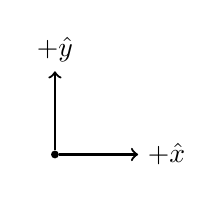
\begin{tikzpicture}
	\node [circle, fill, inner sep = 1pt] (origin) {};
	\node [above = of origin] (y) {$ +\hat{y} $};
	\node [right = of origin] (x) {$ +\hat{x} $};

	\foreach \node in {y, x}
		\draw [black, thick, ->] (origin) -- (\node);
\end{tikzpicture}
\begin{align*}
	m_{(c)ar} & = \SI{950}{\kilogram} \\
	m_{(t)ruck} & = \SI{1900}{\kilogram} \\
	v_1 & = \SI{16.0}{\meter \per \second} \\
	\theta & = \SI{24.0}{\degree \east \of \north} \\
	v_{c_0} & = ? \\
	v_{t_0} & = ?
\end{align*}
Find conservation of momentum in $ \hat{x} $ direction:
\begin{align*}
	v_{c_0} & = v_{c_0}\cos(\SI{0}{\degree}) = v_{c_0} \\
	v_{t_0} & = v_{t_0}\cos(\SI{90.0}{\degree}) = 0 \\
	v_{c_1} & = \SI{16.0}{\meter \per \second}\sin(\SI{24.0}{\degree}) = \SI{6.51}{\meter \per \second} \\
	v_{t_1} & = \SI{16.0}{\meter \per \second}\sin(\SI{24.0}{\degree}) = \SI{6.51}{\meter \per \second}
\end{align*}
\begin{align*}
	P_{0_x} & = P_{1_x} \\
	m_cv_{c_0} + m_tv_{t_0} & = m_cv_{c_1} + m_tv_{t_1} \\
	m_cv_{c_0} + 0 & = v_1 \left( m_c + m_t \right) \\
	v_{c_0} & = \frac{ v_1 \left( m_c + m_t \right) }{ m_c } \\
	v_{c_0} & = \frac{ (\SI{6.51}{\meter \per \second})(\SI{950}{\kilogram} + \SI{1900}{\kilogram}) }{ \SI{950}{\kilogram} } \\
	v_{c_0} & = \SI{19.53}{\meter \per \second}
\end{align*}
Find conservation of momentum in $ \hat{y} $ direction:
\begin{align*}
	v_{c_0} & = v_{c_0}\cos(\SI{90.0}{\degree}) = 0 \\
	v_{t_0} & = v_{t_0}\cos(\SI{0}{\degree}) = v_{t_0} \\
	v_{c_1} & = \SI{16.0}{\meter \per \second}\cos(\SI{24.0}{\degree}) = \SI{14.6}{\meter \per \second} \\
	v_{t_1} & = \SI{16.0}{\meter \per \second}\cos(\SI{24.0}{\degree}) = \SI{14.6}{\meter \per \second}
\end{align*}
\begin{align*}
	m_cv_{c_0} + m_tv_{t_0} & = m_cv_{c_1} + m_tv_{t_1} \\
	0 + m_tv_{t_0} & = v_1(m_c + m_t) \\
	v_{t_0} & = \frac{ v_1(m_c + m_t) }{ m_t } \\
	v_{t_0} & = \frac{ (\SI{14.6}{\meter \per \second})(\SI{950}{\kilogram} + \SI{1900}{\kilogram}) }{ \SI{1900}{\kilogram} } \\
	v_{t_0} & = \SI{21.9}{\meter \per \second}
\end{align*}
\begin{mdframed}
	The speed of the car before collision was $ v_{c_0} = \SI{19.53}{\meter \per \second} $, and the speed of the truck before collision was $ v_{t_0} = \SI{21.9}{\meter \per \second} $.
\end{mdframed}

\subsection{8.44}

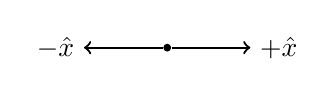
\begin{tikzpicture}
	\node [circle, fill, inner sep = 1pt] (origin) {};
	\node [left = of origin] (x0) {$ -\hat{x} $};
	\node [right = of origin] (x1) {$ +\hat{x} $};

	\foreach \node in {x0, x1}
		\draw[black, thick, ->] (origin) -- (\node);
\end{tikzpicture}
\begin{align*}
	m_{(b)lock} & = \SI{15.0}{\kilogram} \\
	k & = \SI{575.0}{\newton \per \meter} \\
	v_{b_0} & = 0 \\
	m_{(s)tone} & = \SI{3.00}{\kilogram} \\
	v_{s_0} & = \SI{8.00}{\meter \per \second} \\
	v_{s_1} & = \SI{-2.00}{\meter \per \second} \\
	\Delta x_{b,max} & = ?
\end{align*}
Find the velocity of the upon collision $ v_1 $:
\begin{align*}
	P_0 & = P_1 \\
	m_sv_{s_0} + m_bv_{b_0} & = m_sv_{s_1} + m_bv_{b_1} \\
	m_sv_{s_0} + 0 & = m_sv_{s_1} + m_bv_{b_1} \\
	v_{b_1} & = \frac{ m_sv_{s_0} - m_sv_{s_1} }{ m_b } \\
	v_{b_1} & = \frac{ (\SI{3.00}{\kilogram})(\SI{8.00}{\meter \per \second}) - (\SI{3.00}{\kilogram})(\SI{-2.00}{\meter \per \second}) }{ \SI{15.0}{\kilogram} } \\
	v_{b_1} & = \SI{2.00}{\meter \per \second}
\end{align*}
Find the max distance using conservation of energy $ x_{max} $:
\begin{align*}
	E_0 & = E_1 \\
	\frac{1}{2}m_bv_0^2 & = \frac{1}{2}kx_{max}^2 \\
	x_{max} & = \sqrt{ \frac{ m_bv_0^2 }{ k } } \\
	x_{max} & = \sqrt{ \frac{ (\SI{15.0}{\kilogram})(\SI{2.00}{\meter \per \second})^2 }{ \SI{575.0}{\newton \per \meter} } } \\
	x_{max} & = \SI{0.323}{\meter}
\end{align*}
\begin{mdframed}
	The steel ball moves the block to a maximum of $ x_{max} = \SI{0.323}{\meter} $.
\end{mdframed}

\subsection{8.48}

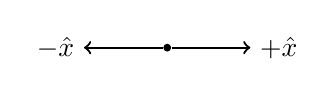
\begin{tikzpicture}
	\node [circle, fill, inner sep = 1pt] (origin) {};
	\node [left = of origin] (x0) {$ -\hat{x} $};
	\node [right = of origin] (x1) {$ +\hat{x} $};

	\foreach \node in {x0, x1}
		\draw[black, thick, ->] (origin) -- (\node);
\end{tikzpicture}
\begin{align*}
	m_{(s)mall} & = \SI{10.0}{\gram} \\
	v_{s_0} & = \SI{-0.400}{\meter \per \second} \\
	m_{(l)arge} & = \SI{30.0}{\gram} \\
	v_{l_0} & = \SI{0.200}{\meter \per \second}
\end{align*}
\begin{enumerate}[label = \textbf{(\alph*)}]
	\item Find the velocity of each marble after the collision. \\
		Since the collision is perfectly elastic, the conservation of momentum and energy both apply. Evaluating each equation will result in two unknowns (the final velocities of the respective marble) which forms a system of equations that can be solved for a single variable, and substituted in the other. * I attempted to use an augmented matrix to solve the system of equations, but was immediately stumped as the conservation of energy equation's unknowns were both squared values which I am unsure of how to handle.
		\begin{align*}
			P_0 & = P_1 \\
			m_sv_{s_0} + m_lv_{l_0} & = m_sv_{s_1} + m_lv_{l_1} \\
			(\SI{10.0}{\gram})(\SI{-0.400}{\meter \per \second}) + (\SI{30.0}{\gram})(\SI{0.200}{\meter \per \second}) & = (\SI{10.0}{\gram})v_{s_1} + (\SI{30.0}{\gram})v_{l_1} \\
			(\SI{10.0}{\gram})v_{s_1} + (\SI{30.0}{\gram})v_{l_1} & = \SI{2.00}{\gram \meter \per \second}
		\end{align*}
		\begin{align*}
			E_0 & = E_1 \\
			\frac{1}{2}m_sv_{s_0}^2 + \frac{1}{2}m_lv_{l_0}^2 & = \frac{1}{2}m_sv_{s_1}^2 + \frac{1}{2}m_lv_{l_1}^2 \\
			(\SI{10.0}{\gram})(\SI{-0.400}{\meter \per \second})^2 + (\SI{30.0}{\gram})(\SI{0.200}{\meter \per \second})^2 & = (\SI{10.0}{\gram})v_{s_1}^2 + (\SI{30.0}{\gram})v_{l_1}^2 \\
			(\SI{10.0}{\gram})v_{s_1}^2 + (\SI{30.0}{\gram})v_{l_1}^2 & = \SI{2.8}{\gram \meter \per \second}
		\end{align*}
		\begin{align*}
			(\SI{10.0}{\gram})v_{s_1} + (\SI{30.0}{\gram})v_{l_1} & = \SI{2.00}{\gram \meter \per \second} \\
			v_{s_1} & = (-3.00)v_{l_1} + \SI{0.200}{\meter \per \second}
		\end{align*}
		\begin{align*}
			(\SI{10.0}{\gram})v_{s_1}^2 + (\SI{30.0}{\gram})v_{l_1}^2 & = \SI{2.8}{\gram \meter \per \second} \\
			(\SI{10.0}{\gram})((-3.00)v_{l_1} + \SI{0.200}{\meter \per \second})^2 + (\SI{30.0}{\gram})v_{l_1}^2 & = \SI{2.8}{\gram \meter \per \second} \\
			(\SI{120.0}{\gram \meter \per \second})v_{l_1}^2 - (\SI{12.0}{\gram \meter \per \second})v_{l_1} - \SI{2.40}{\gram \meter \per \second} & = 0 \\
			v_{l_1} & = \SI{-0.100}{\meter \per \second}, \SI{0.200}{\meter \per \second}
		\end{align*}
		Since the collision is perfectly elastic, the correct value to use for $ v_{l_1} $ would be \SI{-0.100}{\meter \per \second} as the large marble would have to move in the opposite direction ($ -\hat{x} $) of it's initial velocity.
		\begin{align*}
			v_{s_1} & = (-3.00)v_{l_1} + \SI{0.200}{\meter \per \second} \\
			v_{s_1} & = (-3.00)(\SI{-0.100}{\meter \per \second}) + \SI{0.200}{\meter \per \second} \\
			v_{s_1} & = \SI{0.500}{\meter \per \second}
		\end{align*}
		\begin{mdframed}
			Upon collision, the large marble will move \SI{0.100}{\meter \per \second} to the left, while the small marble will move \SI{0.500}{\meter \per \second} to the right.
		\end{mdframed}
	\item Calculate the \textit{change in momentum} for each marble.
		\begin{align*}
			\Delta P_l & = P_{l_1} - P_{l_0} \\
			\Delta P_l & = m_lv_{l_1} - m_lv_{l_0} \\
			\Delta P_l & = (\SI{30.0}{\gram})(\SI{-0.100}{\meter \per \second}) - (\SI{30.0}{\gram})(\SI{0.200}{\meter \per \second}) \\
			\Delta P_l & = \SI{-9.00}{\gram \meter \per \second}
		\end{align*}
		\begin{align*}
			\Delta P_s & = P_{s_1} - P_{s_0} \\
			\Delta P_s & = m_sv_{s_1} - m_sv_{s_0} \\
			\Delta P_s & = (\SI{10.0}{\gram})(\SI{0.500}{\meter \per \second}) - (\SI{10.0}{\gram})(\SI{-0.400}{\meter \per \second}) \\
			\Delta P_s & = \SI{9.00}{\gram \meter \per \second}
		\end{align*}
		\begin{mdframed}
			The change in momentum energy for the large marble is \SI{-9.00}{\gram \meter \per \second} and \SI{9.00}{\gram \meter \per \second} for the small marble.
		\end{mdframed}
	\item Calculate the \textit{change in kinetic energy} for each marble.
		\begin{align*}
			\Delta E_l & = E_{l_1} - E_{l_0} \\
			\Delta E_l & = \frac{1}{2}m_lv_{l_1}^2 - \frac{1}{2}m_lv_{l_0}^2 \\
			\Delta E_l & = \frac{1}{2}(\SI{30.0}{\gram})(\SI{-0.100}{\meter \per \second})^2 - \frac{1}{2}(\SI{30.0}{\gram})(\SI{0.200}{\meter \per \second}) \\
			\Delta E_l & = \SI{-0.450}{\gram \meter \squared \per \second \squared}
		\end{align*}
		\begin{align*}
			\Delta E_s & = E_{s_1} - E_{s_0} \\
			\Delta E_s & = \frac{1}{2}m_sv_{s_1}^2 - \frac{1}{2}m_sv_{s_0}^2 \\
			\Delta E_s & = \frac{1}{2}(\SI{10.0}{\gram})(\SI{0.500}{\meter \per \second})^2 - \frac{1}{2}(\SI{10.0}{\gram})(\SI{-0.400}{\meter \per \second})^2 \\
			\Delta E_s & = \SI{0.450}{\gram \meter \squared \per \second \squared}
		\end{align*}
		\begin{mdframed}
			The change in kinetic energy for the large marble is \SI{-0.450}{\gram \meter \squared \per \second \squared} and \SI{0.450}{\gram \meter \squared \per \second \squared} for the small marble.
		\end{mdframed}
\end{enumerate}

\subsection{8.62}

\begin{align*}
	m_{(f)uel} & = \SI{5.40e-2}{\kilogram \per \second} \\
	v & = \SI{1550}{\meter \per \second}
\end{align*}
\begin{enumerate}[label = \textbf{(\alph*)}]
	\item What is the thrust of the rocket?
		\begin{align*}
			\sum F_{(t)hrust} & = \dot{m}\dot{v} \\
			\sum F_t & = (\SI{5.40e-2}{\kilogram \per \second})(\SI{1550}{\meter \per \second}) \\
			\sum F_t & = \SI{83.7}{\newton}
		\end{align*}
		\begin{mdframed}
			The thrust of the rocket is \SI{83.7}{\newton}.
		\end{mdframed}
	\item Would the rocket operate in outer space where there is no atmosphere? If so, how would you steer it? Could you brake it?
		\begin{mdframed}
			Based on Newton's Third Law (for every force there is an equal and opposite reaction), in order to ``brake" (decelerate) the rocket, all that would be needed is for the rocket to expel fuel in the opposing direction (create an opposing force). The difference that the lack of atmosphere introduces is that the force of gravity from the Earth is much less potent requiring a greater amount of opposing force to decelerate the rocket. Similarly, directing the rocket to a different direction of motion would require that the fuel would be expended at an angle nonparallel to the direction of motion.
		\end{mdframed}
\end{enumerate}

\subsection{8.87}

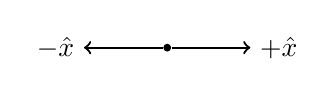
\begin{tikzpicture}
	\node [circle, fill, inner sep = 1pt] (origin) {};
	\node [left = of origin] (x0) {$ -\hat{x} $};
	\node [right = of origin] (x1) {$ +\hat{x} $};

	\foreach \node in {x0, x1}
		\draw[black, thick, ->] (origin) -- (\node);
\end{tikzpicture}
\begin{align*}
	m_{(c)art} & = \SI{50.0}{\kilogram} \\
	v_{c_0} & = \SI{-5.00}{\meter \per \second} \\
	m_{(p)ackage} & = \SI{15.0}{\kilogram} \\
	\theta & = \SI{37}{\degree} \\
	v_{p_0} & = \SI{3.00}{\meter \per \second} \\
	h_0 & = \SI{4.00}{\meter} \\
	h_1 & = 0
\end{align*}
\begin{enumerate}[label = \textbf{(\alph*)}]
	\item What is the speed of the package just before it lands in the cart?
		\begin{align*}
			E_{p_0} & = E_{p_1} \\
			\frac{1}{2}m_pv_{p_0}^2 + m_pgh_0 & = \frac{1}{2}m_pv_{p_1}^2 + m_pgh_1 \\
			v_{p_0}^2 + 2gh_0 & = v_{p_1}^2 + 0 \\
			v_{p_1} & = \sqrt{v_{p_0}^2 + 2gh_0} \\
			v_{p_1} & = \sqrt{(\SI{3.00}{\meter \per \second})^2 + 2(\SI{10.0}{\meter \per \second \squared})(\SI{4.00}{\meter})} \\
			v_{p_1} & = \SI{9.43}{\meter \per \second}
		\end{align*}
		\begin{mdframed}
			The speed of the package before landing is \SI{9.43}{\meter \per \second}.
		\end{mdframed}
	\item What is the final speed of the cart?
		\begin{align*}
			P_{0_x} & = P_{1_x} \\
			m_cv_{c_0} + m_pv_{p_0} & = v_1(m_c + m_p) \\
			v_1 & = \frac{ m_cv_{c_0} + m_pv_{p_0} }{ m_c + m_p } \\
			v_1 & = \frac{ (\SI{50.0}{\kilogram})(\SI{-5.00}{\meter \per \second}) + (\SI{15.0}{\kilogram})(\SI{3.00}{\meter \per \second}\cos(\SI{37.0}{\degree})) }{ \SI{50.0}{\kilogram} + \SI{15.0}{\kilogram} } \\
			v_1 & = \SI{-3.29}{\meter \per \second}
		\end{align*}
		\begin{mdframed}
			The final velocity of the collision results in the collective cart and package moving at \SI{3.29}{\meter \per \second} in the $ -\hat{x} $ direction (left).
		\end{mdframed}
\end{enumerate}

\section{Lab Manual}

\subsection{972}

\begin{enumerate}[label = \textbf{(\alph*)}]
	\item Find the velocity of each body after the collision, in terms of the masses and the velocities given.
		\begin{align*}
			P_0 & = P_1 \\
			m_Av_{A_0} + m_Bv_{B_0} & = m_Av_{A_1} + m_Bv_{B_1} \\
			v_{A_1} & = \frac{ m_Av_{A_0} + m_Bv_{B_0} - m_Bv_{B_1} }{ m_A } \\
			v_{B_1} & = \frac{ m_Av_{A_0} + m_Bv_{B_0} - m_Av_{A_1} }{ m_B }
		\end{align*}
		\begin{align*}
			E_0 & = E_1 \\
			\frac{1}{2}m_Av_{A_0}^2 + \frac{1}{2}m_Bv_{B_0}^2 & = \frac{1}{2}m_Av_{A_1}^2 + \frac{1}{2}m_Bv_{B_1}^2 \\
			v_{A_1} & = \sqrt{ \frac{ m_Av_{A_0}^2 + m_Bv_{B_0}^2 - m_Bv_{B_1}^2 }{ m_A } } \\
			v_{B_1} & = \sqrt{ \frac{ m_Av_{A_0}^2 + m_Bv_{B_0}^2 - m_Av_{A_1}^2 }{ m_B } }
		\end{align*}
		\begin{align*}
			v_{A_1} & = \frac{ m_Av_{A_0} + m_Bv_{B_0} - m_Bv_{B_1} }{ m_A } \\
			v_{A_1} & = \frac{ m_Av_{A_0} + m_Bv_{B_0} - m_B \left( \sqrt{ \frac{ m_Av_{A_0}^2 + m_Bv_{B_0}^2 - m_Av_{A_1}^2 }{ m_B } } \right) }{ m_A } \\
			v_{A_1} & = \frac{ v_{A_0}(m_A - m_B) + 2m_Bv_{B_0} }{ m_A + m_B }
		\end{align*}
		\begin{align*}
			v_{B_1} & = \frac{ m_Av_{A_0} + m_Bv_{B_0} - m_Av_{A_1} }{ m_B } \\
			v_{B_1} & = \frac{ m_Av_{A_0} + m_Bv_{B_0} - m_A \left( \frac{ v_{A_0}(m_A - m_B) + 2m_Bv_{B_0} }{ m_A + m_B } \right) }{ m_B } \\
			v_{B_1} & = \frac{ v_{B_0}(m_B - m_A) + 2m_Av_{A_0} }{ m_A + m_B }
		\end{align*}
		\begin{mdframed}
			The final velocities are
			\begin{align*}
				v_{A_1} & = \frac{ v_{A_0}(m_A - m_B) + 2m_Bv_{B_0} }{ m_A + m_B } \\
				v_{B_1} & = \frac{ v_{B_0}(m_B - m_A) + 2m_Av_{A_0} }{ m_A + m_B }
			\end{align*}
		\end{mdframed}
	\item For the special case in which $ B $ is at rest before collision, find the ratio $$ K = \frac{ \text{Kinetic Energy of $ B $ after collision} }{ \text{Kinetic Energy of $ A $ before collision} } $$, in terms of $ \sfrac{m_A}{m_B} $.
		\begin{align*}
			K & = \frac{ \frac{1}{2}m_Bv_{B_1}^2 }{ \frac{1}{2}m_Av_{A_0}^2 } \\
			K & = \frac{ m_B \left( \frac{ v_{B_0}(m_B - m_A) + 2m_Av_{A_0} }{ m_A + m_B } \right)^2 }{ m_Av_{A_0}^2 } \\
			K & = \frac{ m_B \left( \frac{ (0)(m_B - m_A) + 2m_Av_{A_0} }{ m_A + m_B } \right)^2 }{ m_Av_{A_0}^2 } \\
			K & = \frac{ 4m_Am_B }{ (m_A + m_B)^2 }
		\end{align*}
		\begin{mdframed}
			When $ B $ is at rest before collision, the ratio of kinetic energy is $ K = \frac{ 4m_Am_B }{ (m_A + m_B)^2 } $.
		\end{mdframed}
	\item Let $ r $ stand for the ratio $ \sfrac{m_A}{m_B} $. Find the value of $ r $ that makes $ K(r) $ a maximum. What does $ m_B $ have to be (in terms of $ m_A $) for the maximum transfer of kinetic energy in the collision?
		\begin{align*}
			K & = \frac{ 4m_Am_B }{ m_A^2 + 2m_Am_B + m_B^2 } \\
			K & = \frac{ 4m_Am_B }{ m_B^2 \left( \frac{ m_A^2 }{ m_B^2 } + \frac{ 2m_A }{ m_B } + 1 \right) } \\
			K(r) & = \frac{ 4r }{ r^2 + 2r + 1 } \\
			K' & = - \frac{ 4(r - 1) }{ (r + 1)^3 }
		\end{align*}
		Find when $ K' = 0 $:
		\begin{align*}
			- \frac{ 4(r - 1) }{ (r + 1)^3 } & = 0 \\
			-4r + 4 & = 0 \\
			r & = 1
		\end{align*}
		\begin{mdframed}
			When $ r = 1 $, the function $ K(r) $ is at its maximum.
		\end{mdframed}
\end{enumerate}

\subsection{975}

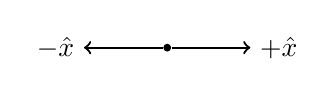
\begin{tikzpicture}
	\node [circle, fill, inner sep = 1pt] (origin) {};
	\node [left = of origin] (x0) {$ -\hat{x} $};
	\node [right = of origin] (x1) {$ +\hat{x} $};

	\foreach \node in {x0, x1}
		\draw[black, thick, ->] (origin) -- (\node);
\end{tikzpicture}
\begin{align*}
	m_A & = \SI{100}{\gram} \\
	v_{\sfrac{A}{E}} & = \SI{10}{\centi \meter \per \second} \\
	m_B & = \SI{50}{\gram} \\
	v_{\sfrac{B}{E}} & = \SI{-8}{\centi \meter \per \second}
\end{align*}
\begin{enumerate}[label = \textbf{(\alph*)}]
	\item Find the velocity of the coupled cars by taking momenta relative to the earth.
		\begin{align*}
			P_0 & = P_1 \\
			m_Av_{\sfrac{A}{E}} + m_Bv_{\sfrac{B}{E}} & = v_{\sfrac{AB}{E}}(m_A + m_B) \\
			v_{\sfrac{AB}{E}} & = \frac{ m_Av_{\sfrac{A}{E}} + m_Bv_{\sfrac{B}{E}} }{ m_A + m_B } \\
			v_{\sfrac{AB}{E}} & = \frac{ (\SI{100}{\gram})(\SI{10}{\centi \meter \per \second}) + (\SI{50}{\gram})(\SI{-8}{\centi \meter \per \second}) }{ \SI{100}{\gram} + \SI{50}{\gram} } \\
			v_{\sfrac{AB}{E}} & = \SI{4.00}{\centi \meter \per \second}
		\end{align*}
	\item Find the velocity of the coupled cars by taking momenta relative to $ B $ (initially).
		\begin{align*}
			v_{\sfrac{AB}{B}} & = v_{\sfrac{AB}{E}} - v_{\sfrac{B}{E}} \\
			v_{\sfrac{AB}{B}} & = \SI{4.00}{\centi \meter \per \second} - (\SI{-8}{\centi \meter \per \second}) \\
			v_{\sfrac{AB}{B}} & = \SI{12.0}{\centi \meter \per \second}
		\end{align*}
	\item \label{975.c} Show that the velocity of the center of mass of the system initially, relative to earth, is \SI{+4}{\centi \meter \per \second}. Then find the velocity of the coupled cars by taking the momenta relative to the center of mass of the system. Why does this result hold for any isolated system, regardless of $ v $'s and $ m $'s?
		\begin{align*}
			v_{CM} & = \sum_{i = 1}^{n} \frac{ p_i }{ m_i } \\
			v_{CM} & = \frac{ m_Av_{\sfrac{A}{E}} + m_Bv_{\sfrac{B}{E}} }{ m_A + m_B } \\
			v_{CM} & = \frac{ (\SI{100}{\gram})(\SI{10}{\centi \meter \per \second}) + (\SI{50}{\gram})(\SI{-8}{\centi \meter \per \second}) }{ \SI{100}{\gram} + \SI{50}{\gram} } \\
			v_{CM} & = \SI{4.00}{\centi \meter \per \second}
		\end{align*}
		\begin{align*}
			P_0 & = P_1 \\
			m_Av_{\sfrac{A}{CM}} + m_Bv_{\sfrac{B}{CM}} & = v_{\sfrac{AB}{CM}}(m_A + m_B) \\
			v_{\sfrac{AB}{CM}} & = \frac{ m_Av_{\sfrac{A}{CM}} + m_Bv_{\sfrac{B}{CM}} }{ m_A + m_B } \\
			v_{\sfrac{AB}{CM}} & = \frac{ (\SI{100}{\gram})(\SI{4.00}{\centi \meter \per \second} - \SI{10}{\centi \meter \per \second}) + (\SI{50}{\gram})(\SI{4.00}{\centi \meter \per \second} - (\SI{-8}{\centi \meter \per \second})) }{ \SI{100}{\gram} + \SI{50}{\gram} } \\
			v_{\sfrac{AB}{CM}} & = 0
		\end{align*}
		As there are no external forces that impact the system, momentum is conserved and is constant. This means that for any velocity vector, there is an opposing vector that will cancel it out and produce a total velocity of zero.
	\item What is the total K.E. of cars $ A $ and $ B $ before and after the collision, and the heart lost in the collision, calculated relative to the center of the earth?
		\begin{align*}
			E_0 & = E_1 \\
			\frac{1}{2}m_Av_{\sfrac{A}{E}}^2 + \frac{1}{2}m_Bv_{\sfrac{B}{E}}^2 & = \frac{1}{2}v_{\sfrac{AB}{E}}^2(m_A + m_B) \\
			(\SI{100}{\gram})(\SI{10}{\centi \meter \per \second})^2 + (\SI{50}{\gram})(\SI{-8}{\centi \meter \per \second})^2 & = (\SI{4.00}{\centi \meter \per \second})^2(\SI{100}{\gram} + \SI{50}{\gram}) \\
			\SI{13200}{\erg} & = \SI{2400}{\erg} \\
			2(\SI{6600}{\erg}) & = 2(\SI{1200}{\erg})
		\end{align*}
		\begin{align*}
			\Delta E & = \left| E_1 - E_0 \right| \\
			\Delta E & = \left| \SI{1200}{\erg} - \SI{6600}{\erg} \right| \\
			\Delta E & = \SI{5400}{\erg}
		\end{align*}
	\item What is the total K.E. of cars $ A $ and $ B $ before and after the collision, and the heat lost, calculated relative to the center of mass of the system?
		\begin{align*}
			E_{{CM}_0} & = \frac{1}{2}m_Av_{\sfrac{A}{CM}}^2 + \frac{1}{2}m_Bv_{\sfrac{B}{CM}}^2 \\
			E_{{CM}_0} & = \frac{1}{2}(\SI{100}{\gram})(\SI{4.00}{\centi \meter \per \second} - \SI{10}{\centi \meter \per \second})^2 + \frac{1}{2}(\SI{50}{\gram})(\SI{4.00}{\centi \meter \per \second} - (\SI{-8}{\centi \meter \per \second}))^2 \\
			E_{{CM}_0} & = \SI{5400}{\erg}
		\end{align*}
		\begin{align*}
			E_{{CM}_1} & = \frac{1}{2}v_{\sfrac{AB}{CM}}(m_A + m_B) \\
			E_{{CM}_1} & = 0
		\end{align*}
		Energy lost to heat would be the difference; \SI{5400}{\erg}.
\end{enumerate}

\subsection{986}

\begin{enumerate}[label = \textbf{(\alph*)}]
	\item
		\begin{align*}
			\theta & = \SI{30.0}{\degree} \\
			\lambda & = \SI{0.50}{\kilogram \per \meter} \\
			v_1 & = \SI{4.0}{\meter \per \second} \\
			m & = \SI{9.0}{\kilogram} \\
			a_1 & = ?
		\end{align*}
		\begin{align*}
			\sum F_x & = \frac{dp}{dt} \\
			mg\sin(\theta) & = \frac{ (m + dm)(v + dv) - mv }{ dt } \\
			mg\sin(\theta) & = \frac{ mv + vdm + mdv + dmdv - mv }{ dt } \\
			mg\sin(\theta) & = v\dot{m} + m\dot{v} \\
			a_x & = g\sin(\theta) - \frac{ \dot{m}v }{ m } \\
			a_x & = (\SI{10}{\meter \per \second \squared})(\sin(\SI{30.0}{\degree})) - \frac{ (\SI{0.50}{\kilogram \per \meter})(\SI{4.0}{\meter \per \second}) }{ \SI{9.0}{\kilogram} }
		\end{align*}
		\bc{ a_x = \SI{4.78}{\meter \per \second \squared} }
	\item
		\begin{enumerate}[label = \textbf{(\arabic*)}]
			\item
				\begin{align*}
					m & = \SI{100}{\kilogram} \\
					v_0 & = \SI{6}{\meter \per \second} \\
					m_1 & = \SI{150}{\kilogram} \\
					v_1 & = ?
				\end{align*}
				\begin{align*}
					\sum F_x & = \frac{dp}{dt} \\
					\frac{m(v + dv) + dmv - m_0v}{dt} & = 0 \\
					m_0dv + vdm & = 0 \\
					-vdm & = m_0dv \\
					- \int_0^m \frac{dm}{m_0} & = \int_{v_0}^v \frac{dv}{v} \\
					-\frac{m}{m_0} & = \ln(v) - \ln(v_0) \\
					\ln(v) & = -\frac{m}{m_0} + \ln(v_0) \\
					\ln(v) & = -\frac{\SI{150}{\kilogram}}{\SI{100}{\kilogram}} + \ln(\SI{6}{\meter \per \second}) \\
					v & = \frac{6}{e^{\sfrac{3}{2}}}
				\end{align*}
			\item
				\begin{align*}
					-\int_0^m \frac{dm}{m_0} & = \int_{v_0}^v \frac{dv}{v} \\
					-\frac{m}{m_0} & = \ln(v) - \ln(v_0) \\
					-\frac{\SI{100}{\kilogram}}{\SI{50}{\kilogram}} & = \ln(v) - \ln(\SI{6}{\meter \per \second}) \\
					v & = \frac{6}{e^2}
				\end{align*}
			\item Because in order to comply with Newton's Third Law, the force the rain temporarily imposes upon the car causes it to decrease in speed.
		\end{enumerate}
\end{enumerate}

\section{Problem B}

Consider a Tsiolkovsky Rocket in a gravitational field, $ g $. At time $ t = 0 $, the velocity of the rocket is $ v = v_0 $, and the mass is $ m = m_0 $. Let the mass loss rate of the rocket be constant in time: $ \dot{m} = -km_0 $ [recall that a variable with a dot on top is the time derivative: $ \dot{m} = \frac{dm}{dt} $, $ \dot{v} = \frac{dv}{dt} $, etc.]
\begin{enumerate}[label = \textbf{\arabic*.}]
	\item Show that the acceleration of the rocket is
		\begin{equation*}
			a = \dot{v} = -\frac{u_{rel}}{m}\dot{m} - g
		\end{equation*}
		\begin{align*}
			F_y & = \frac{dp}{dt} \\
			-g(m + dm) & = m\frac{dv}{dt} + u_{rel}\frac{dm}{dt} \\
			m\frac{dv}{dt} + u_{rel}\frac{dm}{dt} + gm + gdm & = 0 \\
			mdv + u_{rel}dm + gmdt + gdmdt & = 0, \quad dmdt = 0 \\
			mdv + u_{rel}dm + gmdt & = 0 \\
			m\frac{dv}{dt} + u_{rel}\frac{dm}{dt} + gm & = 0 \\
			m\frac{dv}{dt} & = -u_{rel}\frac{dm}{dt} - gm \\
			\dot{v} & = -\frac{u_{rel}}{m}\dot{m} - g
		\end{align*}
		\bc{ a = \dot{v} = -\frac{u_{rel}}{m}\dot{m} - g }
	\item Show that the mass as a function of time is
		\begin{equation*}
			m = m_0(1 - kt)
		\end{equation*}
		\begin{align*}
			\dot{m} & = -km_0 \\
			\int \dot{m} dt & = \int -km_0 dt \\
			m(t) & = -ktm_0 + C \\
			m(0) & = -k(0)m_0 + C = C = m_0, \quad \text{Given from prompt} \\
			m & = -ktm_0 + m_0 = m_0(1 - kt)
		\end{align*}
		\bc{ m = m_0(1 - kt) }
	\item Show that acceleration can also be written as
		\begin{equation*}
			a = \dot{v} = \frac{ku_{rel}}{1 - kt} - g
		\end{equation*}
		\begin{align*}
			a & = -\frac{u_{rel}}{m}\dot{m} - g \\
			a & = -\frac{u_{rel}}{m_0(1 - kt)}(-km_0) - g \\
			a & = \frac{ku_{rel}}{1 - kt} - g
		\end{align*}
		\bc{ a = \frac{ku_{rel}}{1 - kt} - g }
	\item Show that the $ \Delta V $ for a constant mass loss rate rocket is given by:
		\begin{equation*}
			\Delta V = u_{rel}\ln \left[ \frac{1}{1 - kt} \right] - gt
		\end{equation*}
		\begin{align*}
			\int_{0}^{t} (a) dt & = \int_0^{t} \left( \frac{ku_{rel}}{1 - kt} - g \right) dt \\
			\left. V \right|_0^t & = ku_{rel} \int_0^t \left( \frac{1}{1 - kt} \right) dt - \left. gt \right|_0^t \\
			\Delta V & = ku_{rel} \left( \left. \frac{\ln((kt - 1)^{-1})}{k} \right|_0^t \right) - gt \\
			\Delta V & = u_{rel}\ln \left[ \frac{1}{1 - kt} \right] - gt
		\end{align*}
		\bc{ \Delta V = u_{rel}\ln \left[ \frac{1}{1 - kt} \right] - gt }
\end{enumerate}

\end{document}
